\documentclass[aspectratio=169, 11pt]{beamer}

% --- Packages & Setup ---
\usepackage[utf8]{inputenc}
\usepackage[T1]{fontenc}
\usepackage{xcolor}
\usepackage{booktabs} 
\usepackage{graphicx}
\usepackage{amsmath,amssymb}
\usepackage{tikz}
\usetikzlibrary{calc, shapes.geometric, arrows.meta, positioning}

\graphicspath{{../}{./}{images/}}

% Try loading Open Sans; fallback if missing
\IfFileExists{opensans.sty}{\usepackage[default,scale=0.95]{opensans}}{}

% --- Branding Colors ---
\definecolor{amritaMaroon}{HTML}{A4123F} 
\definecolor{darkCharcoal}{HTML}{222222}
\definecolor{accentGold}{HTML}{D4AF37}
\definecolor{lightBg}{HTML}{F8F9FA}
\definecolor{softGreen}{HTML}{2E7D32}

% --- Theme Setup ---
\usetheme{Madrid}
\usecolortheme[named=amritaMaroon]{structure}
\setbeamertemplate{navigation symbols}{}
\setbeamertemplate{footline}[frame number]

% Custom block styles
\setbeamercolor{block title}{bg=amritaMaroon, fg=white}
\setbeamercolor{block body}{bg=amritaMaroon!6, fg=darkCharcoal}
\setbeamercolor{block title example}{bg=darkCharcoal, fg=white}
\setbeamercolor{block body example}{bg=black!5, fg=darkCharcoal}

\begin{document}

% ==============================================================================
% --- TITLE SLIDE ---
% ==============================================================================
\begin{frame}
    % Corner Box Indicator
    \begin{tikzpicture}[remember picture,overlay]
        \node[fill=amritaMaroon, text=white, font=\bfseries\footnotesize, anchor=north east, rounded corners=2pt, inner sep=5pt] 
        at ($(current page.north east) + (-0.2cm,-0.2cm)$) 
        {Type 1: Research Project};
    \end{tikzpicture}

    \centering
    \vspace{0.1cm}
    {\large \textbf{\textcolor{amritaMaroon}{AMRITA VISHWA VIDYAPEETHAM}}} \\
    {\scriptsize School of Computing \quad $\cdot$ \quad Department of Computer Science and Engineering} \\
    \vspace{0.25cm}
    
    {\Large \textbf{\textcolor{amritaMaroon}{Dynamic Task Allocation and Repair Scheduling for Multi-UAV Mobile Edge Computing in FANETs}}} \\
    \vspace{0.1cm}
    {\footnotesize \textbf{23CSE498 -- Project Phase 2 (Panel Review 1)} \quad | \quad \textbf{Team Number: 55}} \\ 
    \vspace{0.2cm}

    % Student Table
    \begin{table}
        \centering
        \footnotesize 
        \renewcommand{\arraystretch}{1.08}
        \begin{tabular}{|c|c|l|}
            \hline
            \textbf{S.No} & \textbf{Register Number} & \textbf{Student Name} \\
            \hline
            1 & CB.EN.U4CSE23337 & Manas Viswajith \\
            \hline
            2 & CB.EN.U4CSE23XXX & Nandagopal Menon \\
            \hline
            3 & CB.EN.U4CSE23XXX & Prabhjot Singh \\
            \hline
            4 & CB.EN.U4CSE23XXX & Student Name 4 \\
            \hline
        \end{tabular}
    \end{table}
    \vspace{0.15cm}
    
    {\footnotesize Guide: \textbf{Faculty Guide Name}, Department of Computer Science and Engineering} \\
    \vspace{0.08cm}
    {\scriptsize \today}
\end{frame}

% ==============================================================================
% --- SLIDE 1(a): METHODOLOGY & MATHEMATICAL MODEL (Rubric: 5 Marks) ---
% ==============================================================================
\section{Methodology \& Solution Design}
\begin{frame}{1(a). Methodology \& Mathematical Formulation}
    \framesubtitle{Rubric: Theoretical Foundation, Mathematical Model \& Evaluation Metrics (5 Marks)}
    \begin{columns}[T]
        % Left Column: System Model & Metrics
        \column{0.48\textwidth}
        \textbf{System Model \& Operational Setup:}
        \begin{itemize}\setlength{\itemsep}{2pt}\footnotesize
            \item \textbf{Terrestrial FANET-MEC:} Multi-UAV airborne edge network serving mobile ground devices (MDs) without centralized cloud infrastructure.
            \item \textbf{Environment Parameters:} 
            \begin{itemize}\scriptsize
                \item 800 MDs distributed across a $2000\text{m} \times 2000\text{m}$ area.
                \item Poisson task arrivals ($\lambda = 1000$ ms per MD).
                \item Swarm of $N$ heterogeneous UAV Fog nodes ($C_j$ queue buffer, $\text{MIPS}_j$ compute capacity).
            \end{itemize}
            \item \textbf{Evaluation Metrics:}
            \begin{itemize}\scriptsize
                \item Scheduling Overhead / Execution Latency (ms).
                \item System Throughput (MB) \& Success Rate (\%).
                \item Drop Rate \& Peer-to-Peer (P2P) Offload Ratio.
            \end{itemize}
        \end{itemize}

        % Right Column: Utility & Constraints
        \column{0.50\textwidth}
        \textbf{Mathematical Formulation:}
        \begin{itemize}\setlength{\itemsep}{2pt}\footnotesize
            \item \textbf{Multi-Objective Utility Function:}
            \vspace{-1.5mm}
            \begin{equation*}
                \small
                U_{ij} = \alpha \left(\frac{1}{1 + d_{ij}^{\text{up}}}\right) + \beta \left(\frac{1}{1 + d_{ij}^{\text{down}}}\right) + \gamma \left(\frac{1}{1 + |\mathcal{Q}_j|}\right)
            \end{equation*}
            \vspace{-2mm}
            \begin{itemize}\scriptsize
                \item $d_{ij}^{\text{up}}, d_{ij}^{\text{down}}$: Uplink/downlink Euclidean distance.
                \item $|\mathcal{Q}_j|$: Current task load on UAV $j$.
                \item Weights: $\alpha=0.4, \beta=0.4, \gamma=0.2$.
            \end{itemize}
            \item \textbf{Feasibility Constraints:}
            \begin{itemize}\scriptsize
                \item \textbf{Latency Deadline:} 
                $T_{ij}^{\text{tx}} + T_{ij}^{\text{queue}} = \frac{D_i}{R_{ij}} + \frac{\sum_{k \in \mathcal{Q}_j} L_k + L_i}{\text{MIPS}_j} \le T_i^{\text{tol}}$
                \item \textbf{Buffer Capacity:} $|\mathcal{Q}_j| \le C_j$ tasks.
                \item \textbf{Coverage Range:} $d_{ij} \le R_{\text{cov}}$ ($130$m).
            \end{itemize}
        \end{itemize}
    \end{columns}
\end{frame}

% ==============================================================================
% --- SLIDE 1(b): SOLUTION DESIGN & ALGORITHMIC WORKFLOW (Rubric: 5 Marks) ---
% ==============================================================================
\begin{frame}{1(b). Solution Design \& Dynamic Repair Workflow}
    \framesubtitle{Rubric: Algorithmic Architecture \& Execution Workflow (5 Marks)}
    \begin{columns}[T]
        % Left Column: Architecture Explanation
        \column{0.44\textwidth}
        \textbf{Dynamic Repair Workflow:}
        \begin{itemize}\setlength{\itemsep}{5pt}\footnotesize
            \item \textbf{1. State Caching:}
            Active task-to-UAV pairings persist in \texttt{AssignmentState} between epochs.
            \item \textbf{2. Selective Invalidation:}
            Prunes only pairings broken by UAV drift ($d > R_{\text{cov}}$) into $\mathcal{A}_{\text{inv}}$.
            \item \textbf{3. Incremental Queue:}
            Merges $\mathcal{A}_{\text{inv}}$ with new arrivals in $\mathcal{Q}_{\text{repair}}$, skipping stable tasks.
            \item \textbf{4. P2P Relaying:}
            Saturated nodes offload to low-load peers within $500$m without global re-matching.
        \end{itemize}

        % Right Column: TikZ Flowchart
        \column{0.56\textwidth}
        \centering
        \vspace{-0.1cm}
        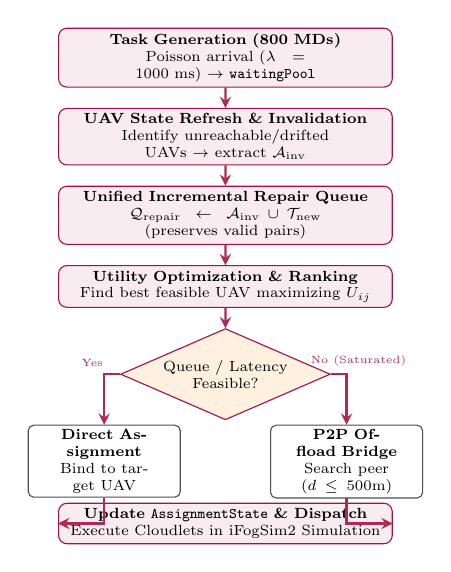
\begin{tikzpicture}[
            scale=0.76, every node/.style={scale=0.76, font=\scriptsize},
            proc/.style={rectangle, draw=amritaMaroon, fill=amritaMaroon!8, rounded corners=3pt, text width=5.4cm, align=center, minimum height=0.48cm, inner sep=2.5pt},
            subproc/.style={rectangle, draw=darkCharcoal!80, fill=white, rounded corners=2pt, text width=2.4cm, align=center, minimum height=0.45cm, inner sep=2pt},
            decision/.style={diamond, draw=amritaMaroon, fill=orange!12, aspect=2.3, text width=2.2cm, align=center, inner sep=1pt},
            arrow/.style={->, >=stealth, thick, color=amritaMaroon!90}
        ]
            % Nodes
            \node[proc] (gen) {\textbf{Task Generation (800 MDs)} \\ Poisson arrival ($\lambda = 1000$ ms) $\to$ \texttt{waitingPool}};
            \node[proc, below=0.26cm of gen] (refresh) {\textbf{UAV State Refresh \& Invalidation} \\ Identify unreachable/drifted UAVs $\to$ extract $\mathcal{A}_{\text{inv}}$};
            \node[proc, below=0.26cm of refresh] (queue) {\textbf{Unified Incremental Repair Queue} \\ $\mathcal{Q}_{\text{repair}} \leftarrow \mathcal{A}_{\text{inv}} \cup \mathcal{T}_{\text{new}}$ (preserves valid pairs)};
            \node[proc, below=0.26cm of queue] (eval) {\textbf{Utility Optimization \& Ranking} \\ Find best feasible UAV maximizing $U_{ij}$};
            \node[decision, below=0.26cm of eval] (dec) {Queue / Latency Feasible?};
            \node[subproc, below left=0.35cm and -0.1cm of dec] (direct) {\textbf{Direct Assignment} \\ Bind to target UAV};
            \node[subproc, below right=0.35cm and -0.1cm of dec] (p2p) {\textbf{P2P Offload Bridge} \\ Search peer ($d \le 500$m)};
            \node[proc, below=1.05cm of dec] (update) {\textbf{Update \texttt{AssignmentState} \& Dispatch} \\ Execute Cloudlets in iFogSim2 Simulation};

            % Arrows
            \draw[arrow] (gen) -- (refresh);
            \draw[arrow] (refresh) -- (queue);
            \draw[arrow] (queue) -- (eval);
            \draw[arrow] (eval) -- (dec);
            \draw[arrow] (dec) -| node[above, font=\tiny, xshift=-0.2cm] {Yes} (direct);
            \draw[arrow] (dec) -| node[above, font=\tiny, xshift=0.2cm] {No (Saturated)} (p2p);
            \draw[arrow] (direct) |- (update);
            \draw[arrow] (p2p) |- (update);
        \end{tikzpicture}
    \end{columns}
\end{frame}

% ==============================================================================
% --- SLIDE 2: IMPLEMENTATION PROGRESS (~60%) (Rubric: 8 Marks) ---
% ==============================================================================
\section{Implementation Progress}
\begin{frame}{2. Implementation Progress ($\approx$60\%) \& Module Functionality}
    \framesubtitle{Rubric: Core Modules Implemented, Functional \& Integrated (8 Marks)}
    \begin{itemize}\setlength{\itemsep}{1pt}
        \item \textbf{Implementation Status Overview ($\approx$60\% Completed -- Phase 2 Milestone 1):}
        \begin{table}
            \centering
            \scriptsize
            \renewcommand{\arraystretch}{1.12}
            \begin{tabular}{p{3.8cm} p{5.2cm} c c}
                \toprule
                \textbf{Module / Component} & \textbf{Technical Implementation State} & \textbf{Progress} & \textbf{Status} \\
                \midrule
                \textbf{FANET MEC Testbed} & Custom iFogSim2 simulation, 800 MDs, Poisson task generation, heterogeneous Fog UAVs & 100\% & Functional \\
                \textbf{Baseline Task Schedulers} & Many-to-One Gale-Shapley (MOGS), Lexicographic Priority, Auction/Bidding, MARL Schedulers & 100\% & Functional \\
                \textbf{Dynamic Repair Engine} & Persistent \texttt{AssignmentState}, selective invalidation, unified incremental repair queue & 100\% & Integrated \\
                \textbf{Cooperative P2P Offload} & Inter-UAV mesh relay for congested Fog nodes ($d \le 500$m) without global re-matching & 100\% & Integrated \\
                \textbf{Benchmarking Pipeline} & Automated Monte Carlo test harness (\texttt{run\_compare.py}), multi-metric regex profiler & 100\% & Functional \\
                \midrule
                \textbf{Phase 2 Remaining Work ($\approx$40\%)} & Topological resilience under extreme churn/node failure, theoretical bounds, paper manuscript & 0\% & Planned \\
                \bottomrule
            \end{tabular}
        \end{table}

        \item \textbf{Core Functionality Demonstration \& Experimental Verification:}
        \begin{itemize}\footnotesize
            \item \textbf{Empirical Validation:} Rigorously benchmarked across 100 independent Monte Carlo simulation runs per scheduler in iFogSim2.
            \item \textbf{Deterministic State Invalidation:} Verified that unaffected UAV assignments remain locked in memory while orphaned tasks are swiftly reallocated.
            \item \textbf{Modular Java Architecture:} Clean decoupled interface (\texttt{TaskScheduler}) allowing hot-swapping between MOGS, Bidding, Lexicographic, and Dynamic Repair.
        \end{itemize}
    \end{itemize}
\end{frame}

% ==============================================================================
% --- SLIDE 3(a): TECHNICAL KNOWLEDGE & FORMULATION (Rubric: 5 Marks) ---
% ==============================================================================
\section{Technical Knowledge}
\begin{frame}{3(a). Technical Knowledge: Algorithmic Rationale \& Formulation}
    \framesubtitle{Rubric: Understanding of Methodology, Implementation \& Design Choices (5 Marks)}
    \begin{columns}[T]
        % Left Column: Limitation of MOGS
        \column{0.48\textwidth}
        \begin{block}{Limitation of MOGS (Gale-Shapley Baseline)}
            \begin{itemize}\setlength{\itemsep}{4pt}\footnotesize
                \item \textbf{Memoryless Recomputation:} Rebuilds preference lists ($M \times N$) from scratch every cycle.
                \item \textbf{Iterative Proposal Overhead:} Multi-round matching ($O(|T| \cdot |U|)$) introduces scheduling jitter on UAV microcontrollers.
                \item \textbf{Unnecessary Churn:} Tiers down and recalculates already stable, valid assignments.
            \end{itemize}
        \end{block}

        % Right Column: Decision for Dynamic Repair
        \column{0.48\textwidth}
        \begin{block}{Decision: Dynamic Matching Maintenance}
            \begin{itemize}\setlength{\itemsep}{4pt}\footnotesize
                \item \textbf{State Persistence:} Active pairings retained in \texttt{AssignmentState} across epochs.
                \item \textbf{Selective Invalidation:} Only disconnects broken links where UAV drifted out of range ($d > R_{\text{cov}}$):
                \vspace{-2mm}
                \begin{equation*}
                    \small
                    \mathcal{A}_{\text{inv}} = \mathcal{A}_{k-1} \setminus \mathcal{A}_{\text{valid}}
                \end{equation*}
                \vspace{-3mm}
                \item \textbf{Unified Repair Queue:} Reallocates only displaced and newly arrived tasks:
                \vspace{-2mm}
                \begin{equation*}
                    \small
                    \mathcal{Q}_{\text{repair}} \leftarrow \mathcal{A}_{\text{inv}} \cup \mathcal{T}_{\text{new}}
                \end{equation*}
            \end{itemize}
        \end{block}
    \end{columns}
\end{frame}

% ==============================================================================
% --- SLIDE 3(b): EMPIRICAL BENCHMARKING & TRADE-OFFS (Rubric: 5 Marks) ---
% ==============================================================================
\begin{frame}{3(b). Design Decisions: Empirical Benchmarks \& Trade-offs}
    \framesubtitle{Rubric: Understanding of Methodology, Implementation \& Design Choices (5 Marks)}
    
    % Centered Benchmark Table with Breathing Room
    \centering
    \footnotesize
    \renewcommand{\arraystretch}{1.2}
    \begin{tabular}{lcccc}
        \toprule
        \textbf{Scheduling Paradigm} & \textbf{Overhead (ms)} & \textbf{Throughput} & \textbf{Success Rate} & \textbf{P2P Offload} \\
        \midrule
        \textbf{Dynamic Repair (Proposed)} & \textbf{0.34 ms} & \textbf{79.5 MB} & \textbf{41.7\%} & \textbf{3.2} \\
        MOGS (Gale-Shapley Baseline)       & 0.67 ms          & 77.9 MB          & 40.9\%          & 3.2 \\
        Lexicographic Priority             & 1.59 ms          & 81.1 MB          & 42.5\%          & 0.0 \\
        Auction / Bidding                  & 29.13 ms         & 72.2 MB          & 37.9\%          & 0.0 \\
        MARL Allocation                    & 19.49 ms         & 6.8 MB           & 3.6\%           & 0.0 \\
        \bottomrule
    \end{tabular}
    \vspace{0.3cm}

    % Concise, Punchy Takeaways
    \begin{itemize}\setlength{\itemsep}{6pt}\small
        \item \textbf{$>$50\% Overhead Reduction:} Slashes scheduling latency from $0.67\text{ ms}$ to $0.34\text{ ms}$ per batch (and up to $85\times$ faster than Bidding) for real-time edge viability.
        \item \textbf{Zero Throughput Loss:} Achieves throughput parity ($79.5\text{ MB}$ vs $77.9\text{ MB}$) without redundant preference recalculation.
        \item \textbf{Seamless Load Balancing:} Fully preserves cooperative P2P offloading ($3.2$ tasks/run) without iterative multi-round matching overhead.
    \end{itemize}
\end{frame}

% ==============================================================================
% --- SLIDE 4: TECHNICAL ENRICHMENT ACTIVITY CHOICES ---
% ==============================================================================
\section{Technical Enrichment}
\begin{frame}{4. Technical Enrichment Activity Choices}
    \framesubtitle{Professional Online Certification Details (Individual Mandatory: 10--20 Hours)}
    \begin{itemize}
        \item \textbf{Individual MOOC / Online Certification Selection (Domain-Aligned):}
    \end{itemize}
    \vspace{-0.15cm}
    \begin{table}
        \centering
        \footnotesize
        \renewcommand{\arraystretch}{1.18}
        \begin{tabular}{|c|p{2.8cm}|p{5.2cm}|p{2.3cm}|c|}
            \hline
            \textbf{S.No} & \textbf{Student Name} & \textbf{Chosen MOOC / Course Title} & \textbf{Platform} & \textbf{Hours} \\
            \hline
            1 & Manas Viswajith & Cloud Computing and Distributed Systems & NPTEL / Swayam & 20 Hrs \\
            \hline
            2 & Nandagopal Menon & Edge Computing and IoT Systems Architecture & Coursera & 16 Hrs \\
            \hline
            3 & Prabhjot Singh & Game Theory and Algorithmic Mechanism Design & NPTEL & 20 Hrs \\
            \hline
            4 & Student Name 4 & Wireless Ad-Hoc and Sensor Networks & Coursera / edX & 15 Hrs \\
            \hline
        \end{tabular}
    \end{table}
    \vspace{0.15cm}
    \begin{itemize}\footnotesize
        \item \textbf{Curricular Relevance:} Selected certifications provide theoretical grounding in distributed consensus, fog computing resource management, and algorithmic game theory directly applicable to Phase 2 objectives.
    \end{itemize}
\end{frame}

% ==============================================================================
% --- REFERENCES ---
% ==============================================================================
\section{References}
\begin{frame}{References}
    \footnotesize
    \begin{thebibliography}{9}
        \bibitem{mahmud2022ifogsim2}
        R.~Mahmud, S.~Pallewatta, M.~Goudarzi, and R.~Buyya, 
        \newblock ``iFogSim2: An extended iFogSim simulator for mobility, clustering, and microservice management in edge and fog computing environments,'' 
        \newblock \emph{Journal of Systems and Software}, vol. 190, p. 111351, 2022.

        \bibitem{zhao2025multi}
        M.~Zhao, F.~Tang, T.~Tan, L.~Luo, and Z.~Guo, 
        \newblock ``A Multi-UAV Cooperative Task Scheduling in Dynamic Environments: Throughput Maximization,'' 
        \newblock \emph{IEEE Internet of Things Journal}, vol. 12, no. 4, pp. 3120--3134, 2025.

        \bibitem{gale1962college}
        D.~Gale and L.~S. Shapley, 
        \newblock ``College admissions and the stability of marriage,'' 
        \newblock \emph{The American Mathematical Monthly}, vol. 69, no. 1, pp. 9--15, 1962.

        \bibitem{mao2017survey}
        Y.~Mao, C.~You, J.~Zhang, K.~Huang, and K.~B. Letaief, 
        \newblock ``A survey on mobile edge computing: The communication perspective,'' 
        \newblock \emph{IEEE Communications Surveys \& Tutorials}, vol. 19, no. 4, pp. 2322--2358, 2017.
    \end{thebibliography}
\end{frame}

% ==============================================================================
% --- THANK YOU SLIDE ---
% ==============================================================================
\begin{frame}
    \centering    
    \vspace{0.8cm}
    {\Huge \textbf{\textcolor{amritaMaroon}{Thank You}}} \\
    \vspace{0.4cm}
    {\large \textbf{Questions \& Discussion}} \\
    \vspace{0.3cm}
    {\footnotesize \textbf{Project Phase 2 -- Panel Review 1} \quad | \quad Team 55} \\
    \vspace{0.2cm}
    {\scriptsize Department of Computer Science and Engineering, Amrita Vishwa Vidyapeetham}
\end{frame}

\end{document}
